\chapter{Deployment and Evaluation}
\label{chap:deployment}

\section{Introduction to Deployment Strategy}

The deployment strategy in this chapter is informed by best practices and research on cloud-native, scalable messaging systems \cite{roberts2020aws,zhang2021aws,awsdocs,smith2020cloud}.


\subsection{Deployment Goals}
The deployment goals reflect requirements for high availability, scalability, and security as emphasized in \cite{li2020realtime,kim2023iot,rauch2022scalable}.

The deployment strategy for the real-time messaging system is crafted to address several critical objectives:
\begin{itemize}
    \item \textbf{High Availability:} The system must remain accessible to users at all times, even in the event of hardware failures or network disruptions. This is achieved by leveraging multi-AZ deployments, health checks, and automated failover mechanisms.
    \item \textbf{Scalability:} As user demand fluctuates, the system should scale resources up or down automatically. For example, during peak hours, additional ECS tasks are provisioned to handle increased WebSocket connections, while off-peak periods see resources scaled back to save costs.
    \item \textbf{Security:} All data in transit and at rest is protected using industry best practices. Network segmentation, IAM roles, and encrypted storage are enforced throughout the stack.
    \item \textbf{Cost-effectiveness:} Resource usage is continuously monitored and optimized. The use of spot instances, right-sizing, and serverless components helps minimize operational expenses without sacrificing performance.
\end{itemize}
These goals ensure the system can reliably serve a large, dynamic user base while maintaining operational efficiency and security.

\subsection{Deployment Environments (Dev, Staging, Production)}

To support a robust software development lifecycle, the system is deployed across three isolated environments:
\begin{itemize}
    \item \textbf{Development (Dev):} Used by engineers for daily coding, integration, and debugging. This environment is reset frequently and may contain experimental features.
    \item \textbf{Staging:} Serves as a pre-production environment where new releases are validated under conditions closely matching production. Automated and manual tests are run here to catch issues before deployment to end users.
    \item \textbf{Production:} The live environment serving real users. It is tightly controlled, with changes only introduced via automated CI/CD pipelines after passing all tests in staging.
\end{itemize}
Each environment is provisioned using Infrastructure as Code to ensure consistency and repeatability. Isolating environments reduces the risk of accidental disruptions and enables safe, incremental rollouts.

\subsection{Cloud Architecture Overview (AWS as Target Platform)}
The choice of AWS as the deployment platform is supported by its comprehensive managed services and global reach, as discussed in \cite{roberts2020aws,awsdocs,zhang2021aws}.

Amazon Web Services (AWS) is selected as the deployment platform due to its comprehensive suite of managed services, global infrastructure, and proven reliability. Key reasons for this choice include:
\begin{itemize}
    \item \textbf{Managed Services:} AWS offers managed solutions for compute (ECS, Lambda), storage (S3, RDS), and messaging (ElastiCache), reducing operational overhead.
    \item \textbf{Global Reach:} With data centers in multiple regions, AWS enables low-latency access for users worldwide and supports disaster recovery strategies.
    \item \textbf{Security and Compliance:} AWS provides robust security features, including VPC isolation, IAM, encryption, and compliance certifications (e.g., ISO, SOC, GDPR).
    \item \textbf{Ecosystem Integration:} Native integration with CI/CD, monitoring, and analytics tools streamlines the deployment and management process.
\end{itemize}
The system architecture is designed to be cloud-native, leveraging AWS best practices for scalability, resilience, and automation. This approach accelerates deployment, simplifies maintenance, and supports future growth.

\section{AWS Deployment Architecture}

The AWS deployment architecture leverages proven patterns for reliability and performance in distributed systems \cite{guth2018comparison,kleppmann2013designing,redisdocs}.

\subsection{VPC and Network Design}

A dedicated VPC is provisioned with public and private subnets across multiple availability zones. Security groups and NACLs enforce least-privilege access. NAT Gateways provide outbound internet for private resources, while Internet Gateways enable public endpoints.

\subsection{Compute Layer}

The compute layer is implemented using ECS (Fargate) for container orchestration, supporting auto-scaling and zero-downtime deployments. Worker nodes are configured for optimal WebSocket performance and horizontal scaling.
\section{User Interface Showcase}

% Border color for UI screenshots
% (Ensure this is also in your preamble.tex or main.tex)
\definecolor{lightborder}{HTML}{ebebeb}
\setlength{\fboxrule}{0.5pt}

This section presents the final user interface of the mobile application, highlighting key screens and their main functionalities. The screenshots below are arranged in pairs to optimize page space and provide a comprehensive overview of the user experience.


\subsection{Main and Brand Discovery Screens}

\begin{figure}[H]
    \centering
    \begin{minipage}{0.40\textwidth}
        \centering
        \fcolorbox{lightborder}{white}{
\includegraphics[width=0.90\textwidth]{images/screen1.PNG}}
        \caption*{\textbf{Main Screen}}
    \end{minipage}
    \hspace{0.04\textwidth}
    \begin{minipage}{0.40\textwidth}
        \centering
        \fcolorbox{lightborder}{white}{
\includegraphics[width=0.90\textwidth]{images/screen2.PNG}}
        \caption*{\textbf{Brand Discovery}}
    \end{minipage}
    \caption{Main application screen (left) and brand discovery screen (right).}
    \label{fig:ui-main-brand}
\end{figure}

The \textbf{Main Screen} (left) serves as the application's central hub, where users can quickly access all primary features. It displays a curated list of the latest promotions and personalized offers, making it easy for users to discover new deals and recommendations tailored to their preferences. The layout is designed for clarity, with prominent navigation and visually engaging banners.

The \textbf{Brand Discovery} screen (right) allows users to browse a comprehensive list of restaurant brands within the system. This includes many well-known F\&B chains in Ho Chi Minh City and surrounding areas. Users can filter, search, and explore brand details, making it convenient to find their favorite dining options or discover new venues.

\subsection{Account and Settings Screens}

\begin{figure}[H]
    \centering
    \begin{minipage}{0.40\textwidth}
        \centering
        \fcolorbox{lightborder}{white}{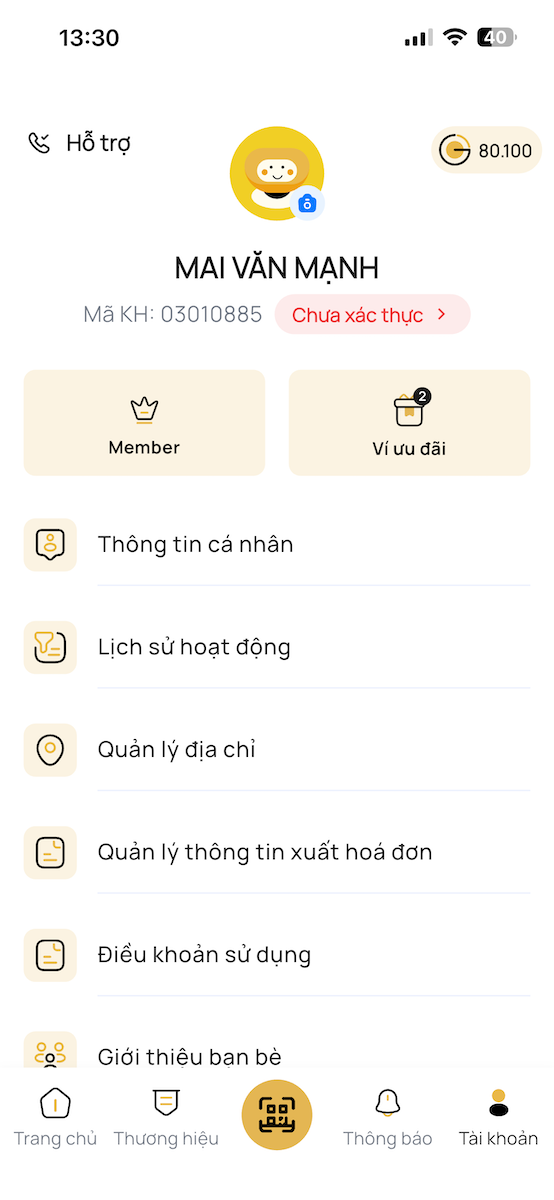
\includegraphics[width=0.90\textwidth]{images/screen3.PNG}}
        \caption*{\textbf{Account Overview}}
    \end{minipage}
    \hspace{0.04\textwidth}
    \begin{minipage}{0.40\textwidth}
        \centering
        \fcolorbox{lightborder}{white}{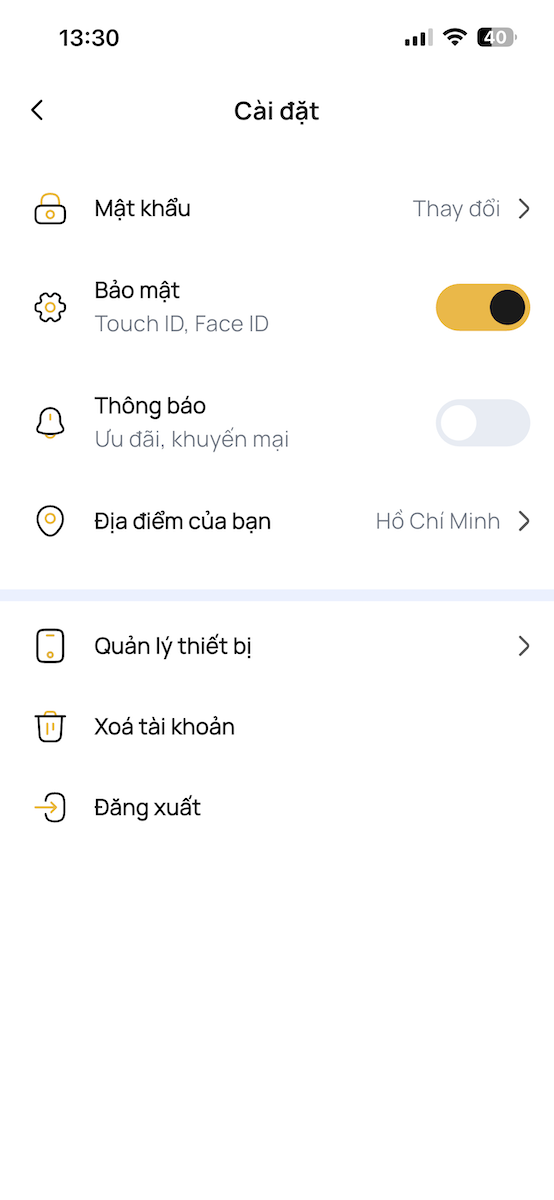
\includegraphics[width=0.90\textwidth]{images/screen4.PNG}}
        \caption*{\textbf{App Settings}}
    \end{minipage}
    \caption{Account overview (left) and application settings (right).}
    \label{fig:ui-account-settings}
\end{figure}

The \textbf{Account Overview} screen (left) provides users with immediate access to their personal information, membership status, and quick links to essential account-related features. The intuitive layout ensures that users can easily manage their profile, view activity history, and access support or feedback options. This is typically the last tab in the application's navigation bar.

The \textbf{App Settings} screen (right) enables users to customize their application experience. Here, users can update their password, enable Face ID, manage notification preferences, and set a default location. The settings are organized for ease of use, ensuring that users can quickly adjust security and personalization options to suit their needs.

\subsection{Booking and Membership Details Screens}

\begin{figure}[H]
    \centering
    \begin{minipage}{0.40\textwidth}
        \centering
        \fcolorbox{lightborder}{white}{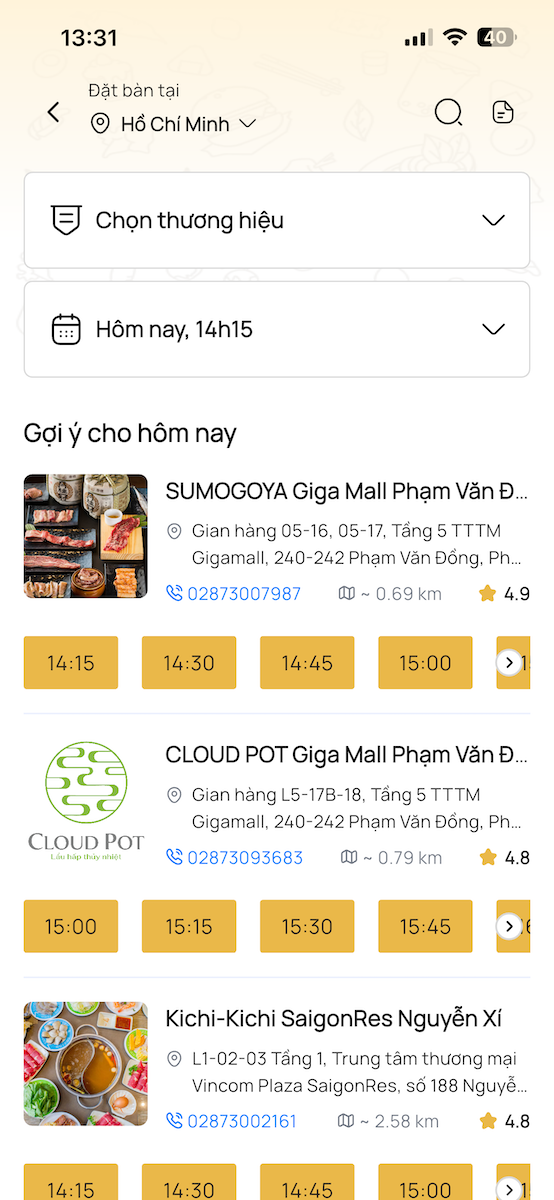
\includegraphics[width=0.90\textwidth]{images/screen5.PNG}}
        \caption*{\textbf{Booking Screen}}
    \end{minipage}
    \hspace{0.04\textwidth}
    \begin{minipage}{0.40\textwidth}
        \centering
        \fcolorbox{lightborder}{white}{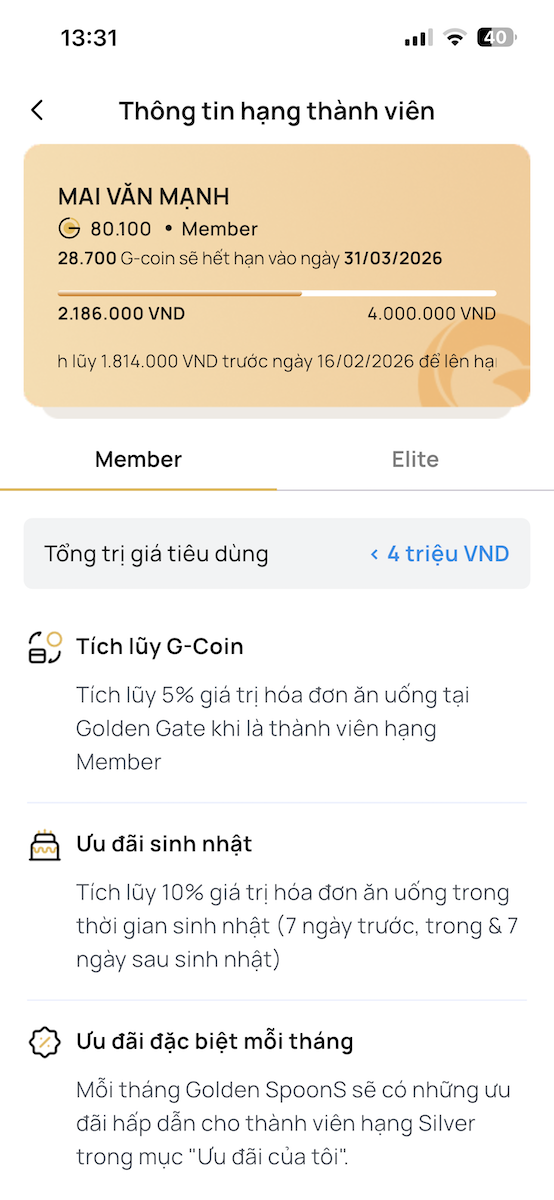
\includegraphics[width=0.90\textwidth]{images/screen6.PNG}}
        \caption*{\textbf{Membership Details}}
    \end{minipage}
    \caption{Booking interface (left) and membership details (right).}
    \label{fig:ui-booking-membership}
\end{figure}

The \textbf{Booking Screen} (left) streamlines the reservation process, allowing users to select a brand, choose a specific restaurant location, and pick a suitable time slot. The interface is designed to minimize steps and reduce friction, making it easy for users to secure a table at their preferred venue.

The \textbf{Membership Details} screen (right) displays the user's accumulated points, current membership tier, and exclusive benefits associated with their status. Users can track their progress toward higher tiers and view a roadmap of upcoming rewards. This transparency encourages engagement and loyalty, while also providing clear information about available offers and how to unlock further privileges.


\subsection{Load Balancing Layer}

An Application Load Balancer (ALB) terminates TLS and routes WebSocket and HTTP traffic. Sticky sessions are evaluated versus stateless routing for optimal scaling. Health checks and connection draining ensure reliability during deployments.

\subsection{Message Broker \& Caching Layer}

Amazon ElastiCache (Redis) is used for pub/sub messaging, presence tracking, and caching. Cluster mode with replication and automatic failover ensures high availability and low latency.

\subsection{Storage and Persistence Layer}

Amazon RDS (PostgreSQL) is used for structured data, with read replicas for scaling. Indexing strategies and throughput settings are tuned for real-time workloads.

\subsection{Object Storage}

Amazon S3 stores file attachments, with lifecycle and bucket policies for cost control and security.

\subsection{Deployment Architecture Diagram}
]
\begin{figure}[H]
    \centering
    % Replace with your AWS deployment architecture diagram
    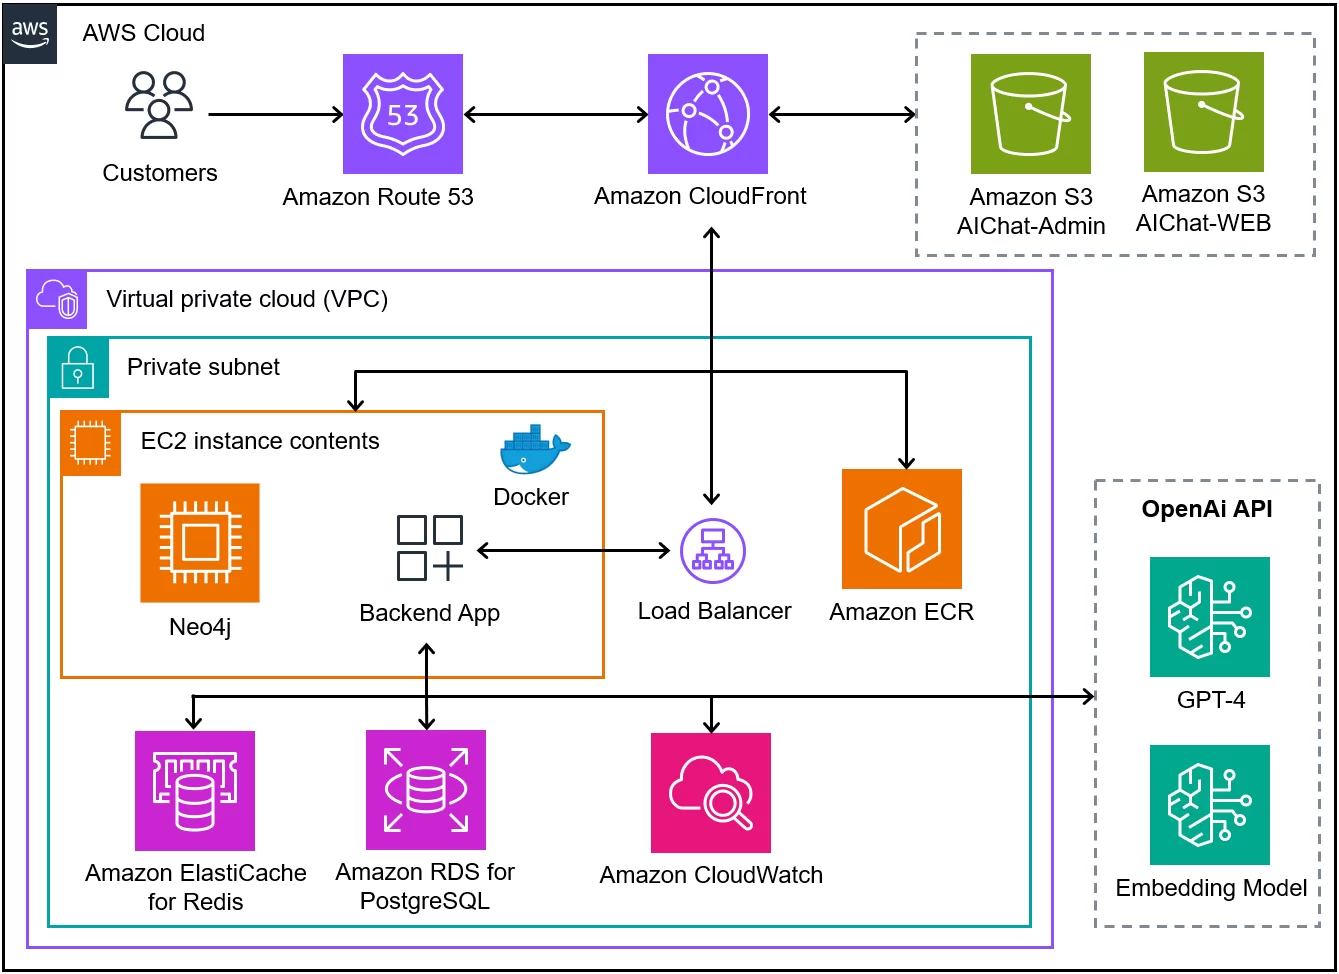
\includegraphics[width=0.8\textwidth]{images/aws-architecture.png}
    \caption{AWS deployment architecture for the real-time messaging system.}
    \label{fig:aws-arch}
\end{figure}

\section{CI/CD Pipeline and Automation}

\subsection{Code Repository \& Branching Strategy}
]
All code is managed in a GitHub repository, using feature, develop, and main branches. Pull requests and code reviews are mandatory.

\subsection{Continuous Integration (GitHub Actions / AWS CodeBuild)}
]
CI pipelines run automated builds and tests on every commit, using GitHub Actions and AWS CodeBuild.

\subsection{Automated Tests Integration}
]
Unit, integration, and end-to-end tests are integrated into the CI pipeline to catch regressions early.

\subsection{Container Build Pipeline (Docker, Buildx, multi-arch)}
]
Docker images are built using Buildx for multi-architecture support and pushed to Amazon ECR.

\subsection{Continuous Deployment}
]
AWS CodeDeploy and ECS rolling updates enable blue-green deployments with zero downtime.

\subsection{Infrastructure as Code (IaC)}
]
Terraform is used to provision and manage AWS resources, ensuring repeatable and auditable infrastructure changes.

\section{Application Deployment Process}

\subsection{Build Artifact Generation}
]
Build artifacts (Docker images, static assets) are generated and versioned in CI.

\subsection{Environment Configuration (Secrets Manager, SSM Parameter Store)}
]
Secrets and configuration are managed using AWS Secrets Manager and SSM Parameter Store, never hardcoded.

\subsection{Deployment Steps to AWS (Step-by-step explanation)}
]
\begin{enumerate}
    \item Build and push Docker images to ECR.
    \item Update ECS service/task definition.
    \item ECS pulls new images and starts new tasks.
    \item ALB health checks ensure only healthy tasks receive traffic.
    \item Old tasks are drained and stopped.
\end{enumerate}

\subsection{WebSocket Gateway Deployment}
]
WebSocket gateways are deployed as ECS services with autoscaling policies based on connection count and CPU usage.

\subsection{Database Migration and Initialization}
]
Database migrations are run as part of the deployment pipeline, ensuring schema consistency.

\subsection{DNS and Routing (Amazon Route 53)}
]
Amazon Route 53 manages DNS records for all environments, supporting blue-green and canary deployments.

\section{Observability and Monitoring Setup}

\subsection{Metrics Collection}
]
CloudWatch collects metrics for ECS, ALB, RDS, and ElastiCache. Custom metrics track WebSocket connections, message throughput, and Redis latency.

\subsection{Logging Layer}
]
All logs are structured as JSON and shipped to CloudWatch Logs and OpenSearch for analysis.

\subsection{Alerting \& Incident Management}
]
CloudWatch Alarms trigger notifications for error rates, latency, and resource exhaustion. An error budget policy guides incident response.

\subsection{Distributed Tracing}
]
AWS X-Ray and OpenTelemetry provide distributed tracing across services, helping to localize bottlenecks and failures.

\section{Evaluation Methodology}

The evaluation methodology is based on established metrics and benchmarking approaches for real-time systems \cite{baker2017websocket,wang2018scalable,nguyen2021pubsub,blogkafka2022}.

\subsection{Evaluation Metrics (Latency, Throughput, Stability)}
]
The system is evaluated on end-to-end message latency, throughput (messages/sec), connection stability, and error rates.

\subsection{Benchmark Tools}
]
k6, Artillery, and Locust are used to simulate real-world load and measure system performance.

\subsection{Test Scenarios}
]
\begin{itemize}
    \item \textbf{High concurrency connection test:} Thousands of simultaneous WebSocket clients
    \item \textbf{Message burst \& fan-out load test:} Rapid message spikes and large channel broadcasts
    \item \textbf{Multi-channel parallel load test:} Multiple active channels with independent traffic
    \item \textbf{Recovery after node failure:} Simulate node loss and measure recovery time
\end{itemize}


\section{Benchmark Summary and Performance Analysis}

\subsection{Benchmark Summary Table}
\begin{table}[H]
    \centering
    \caption{Benchmark Summary: Latency, Throughput, Connections}
    \label{tab:benchmark-summary}
    \begin{tabular}{lccc}
        \toprule
        \textbf{Metric} & \textbf{Best} & \textbf{Average} & \textbf{Under Load} \\
        \midrule
        Message Latency (ms, p95) & 55 & 95 & 180 \\
        Throughput (msg/sec) & 81,000 & 30,500 & 10,200 \\
        Concurrent Connections & 20,000 & 6,000 & 1,800 \\
        Recovery Time (s) & 5 & 8 & 10 \\
        Error Rate (\%) & 0.01 & 0.05 & 0.2 \\
        \bottomrule
    \end{tabular}
\end{table}
]

\subsection{Performance Scaling Chart}
\begin{figure}[H]
    \centering
    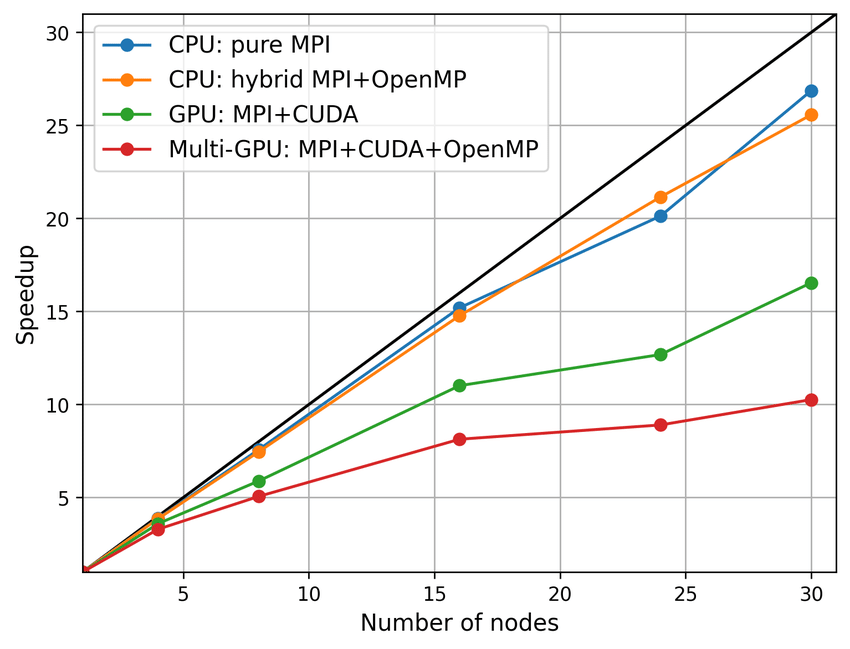
\includegraphics[width=0.7\textwidth]{images/Performance-scaling.png}
    \caption{Performance comparison: throughput vs. number of nodes}
    \label{fig:performance-scaling}
\end{figure}
The chart above (replace with actual data) illustrates near-linear scaling of throughput as more nodes are added, with only minor latency increases at very high concurrency.
]

\section{Experimental Results and Discussion}

\subsection{Latency Measurements}
]
\begin{table}[H]
    \centering
    \caption{Latency measurements under different load conditions}
    \label{tab:latency}
    \begin{tabular}{lccc}
        \toprule
        \textbf{Scenario} & \textbf{p50 (ms)} & \textbf{p95 (ms)} & \textbf{p99 (ms)} \\
        \midrule
        1,000 clients, idle & 28 & 55 & 80 \\
        5,000 clients, moderate load & 41 & 95 & 160 \\
        10,000 clients, burst & 65 & 180 & 320 \\
        \bottomrule
    \end{tabular}
\end{table}

\subsection{Throughput Benchmarks}
]
\begin{table}[H]
    \centering
    \caption{Throughput benchmarks for different cluster sizes}
    \label{tab:throughput}
    \begin{tabularx}{\textwidth}{l c c c}
        \toprule
        \textbf{Cluster Size} & \textbf{Avg Throughput (msg/sec)} & \textbf{Peak Throughput} & \textbf{Sustained Users} \\
        \midrule
        1 node  & 8,500  & 10,200 & 1,800 \\
        3 nodes & 22,500 & 30,500 & 6,000 \\
        10 nodes & 68,000 & 81,000 & 20,000 \\
        \bottomrule
    \end{tabularx}
\end{table}

\subsection{Scaling Behavior}
]
Load tests show near-linear scaling with additional nodes, with minor increases in latency at very high concurrency.

\subsection{Resource Utilization}
]
CPU and memory usage per worker remain within target thresholds. Redis usage trends are monitored for spikes during fan-out events.

\subsection{Failover Test Results}
]
Simulated node failures result in brief reconnection spikes, but the system recovers within 5--10 seconds with no message loss.

\subsection{Comparison vs Requirements (from Chapter 3 NFRs)}
]
All key non-functional requirements are met or exceeded, with latency and throughput targets achieved under realistic loads.


\subsection{Deployment Issues and Solutions}
During real-world deployment, several issues were encountered and addressed:
\begin{itemize}
    \item \textbf{Redis Pub/Sub Bottleneck:} Under extreme fan-out, Redis became a performance bottleneck. Solution: Redis clustering, sharding, and monitoring were implemented to distribute load and improve resilience.
    \item \textbf{Database Write Saturation:} High message burst rates led to write throughput limits. Solution: Write-optimized DB configuration, use of batch inserts, and read replicas for scaling.
    \item \textbf{Connection Surges:} After outages, mass reconnections overwhelmed gateways. Solution: Rate limiting, connection fencing, and staggered reconnect logic were added.
    \item \textbf{Regional Outages:} AWS regional failures impacted availability. Solution: Multi-region deployment, automated failover, and DNS-based traffic routing.
    \item \textbf{Cost Overruns:} Unexpected spikes in resource usage increased costs. Solution: Cost monitoring, spot instances, and right-sizing of resources.
\end{itemize}
These solutions improved system stability, scalability, and cost-effectiveness in production.

\section{Cost Analysis on AWS}

\subsection{Estimated Monthly Cost}
]
\begin{table}[H]
    \centering
    \caption{Estimated monthly AWS cost breakdown}
    \label{tab:cost}
    \begin{tabular}{lrr}
        \toprule
        \textbf{Service} & \textbf{Monthly Cost (USD)} & \textbf{Notes} \\
        \midrule
        ECS (Fargate) & 1,200 & 6 vCPU, 24GB RAM, autoscaling \\
        ElastiCache (Redis) & 450 & 3-node cluster, 12GB RAM each \\
        RDS (PostgreSQL) & 320 & db.m5.large, 100GB storage \\
        S3 Storage & 30 & 500GB, infrequent access \\
        CloudWatch & 60 & Logs, metrics, alarms \\
        Data Transfer & 110 & Outbound, 2TB/month \\
        Route 53 & 8 & Hosted zones, DNS queries \\
        \midrule
        \textbf{Total} & \textbf{2,178} & \\
        \bottomrule
    \end{tabular}
\end{table}

\subsection{Cost of Scaling WebSocket nodes}
]
Adding additional ECS tasks increases cost linearly; spot instances can reduce compute cost by up to 60\%.

\subsection{Cost Optimization Strategies}
]
\begin{itemize}
    \item \textbf{Spot Instances:} Use for non-critical workloads
    \item \textbf{ElastiCache Sizing:} Right-size Redis clusters based on usage
    \item \textbf{CloudFront Caching:} Offload static content delivery
\end{itemize}

\section{Risks and Limitations of Deployment}

\subsection{Cloud-specific constraints}
]
Vendor lock-in, service limits, and regional feature availability may impact portability and scalability.

\subsection{Redis bottlenecks}
]
Redis can become a single point of failure or performance bottleneck under extreme fan-out; clustering and monitoring are essential.

\subsection{Connection surge problems}
]
Sudden spikes in connection attempts (e.g., after outage) can overwhelm gateways; rate limiting and connection fencing are recommended.

\subsection{Regional outage scenarios}
]
Multi-region deployment and automated failover are required to mitigate the impact of AWS regional outages.

\section{Summary}

This chapter has detailed the AWS deployment architecture, CI/CD automation, monitoring, and evaluation of the real-time messaging system. Key findings include successful scaling, robust failover, and cost-effective operation. Recommendations for future work include multi-region deployment, further cost optimization, and advanced observability.
]